\hypertarget{main_8cpp}{
\section{main.cpp File Reference}
\label{main_8cpp}\index{main.cpp@{main.cpp}}
}
Das main Initialisiert das Programm und erstellt den Hauptdialog. 

{\tt \#include \char`\"{}beo\_\-timing.h\char`\"{}}\par
{\tt \#include \char`\"{}logondialog.h\char`\"{}}\par
{\tt \#include $<$QtGui$>$}\par
{\tt \#include $<$QApplication$>$}\par
{\tt \#include $<$QtDebug$>$}\par
{\tt \#include $<$iostream$>$}\par


Include dependency graph for main.cpp:\nopagebreak
\begin{figure}[H]
\begin{center}
\leavevmode
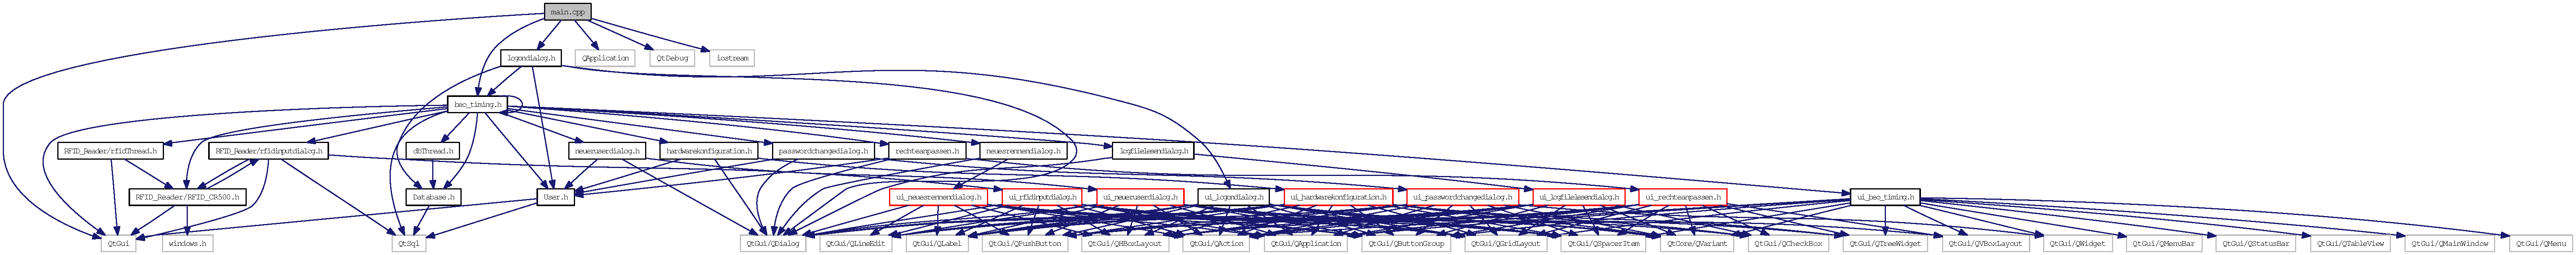
\includegraphics[width=420pt]{main_8cpp__incl}
\end{center}
\end{figure}
\subsection*{Functions}
\begin{CompactItemize}
\item 
int \hyperlink{main_8cpp_0ddf1224851353fc92bfbff6f499fa97}{main} (int argc, char $\ast$argv\mbox{[}$\,$\mbox{]})
\end{CompactItemize}


\subsection{Detailed Description}
Das main Initialisiert das Programm und erstellt den Hauptdialog. 

\begin{Desc}
\item[Version:]1.0 \end{Desc}
\begin{Desc}
\item[Date:]09.06.2008 \end{Desc}
\begin{Desc}
\item[Author:]R.Zoss\end{Desc}
Copyright (C) 2008 Rico Zoss

This file is part of BEO-Timing Managementsoftware.

BEO-Timing Managementsoftware is free software: you can redistribute it and/or modify it under the terms of the GNU General Public License as published by the Free Software Foundation, either version 3 of the License, or (at your option) any later version.

BEO-Timing Managementsoftware is distributed in the hope that it will be useful, but WITHOUT ANY WARRANTY; without even the implied warranty of MERCHANTABILITY or FITNESS FOR A PARTICULAR PURPOSE. See the GNU General Public License for more details.

You should have received a copy of the GNU General Public License along with BEO-Timing Managementsoftware. If not, see $<$\href{http://www.gnu.org/licenses/}{\tt http://www.gnu.org/licenses/}$>$. 

Definition in file \hyperlink{main_8cpp-source}{main.cpp}.

\subsection{Function Documentation}
\hypertarget{main_8cpp_0ddf1224851353fc92bfbff6f499fa97}{
\index{main.cpp@{main.cpp}!main@{main}}
\index{main@{main}!main.cpp@{main.cpp}}
\subsubsection[main]{\setlength{\rightskip}{0pt plus 5cm}int main (int {\em argc}, \/  char $\ast$ {\em argv}\mbox{[}$\,$\mbox{]})}}
\label{main_8cpp_0ddf1224851353fc92bfbff6f499fa97}




Definition at line 43 of file main.cpp.